\documentclass[11pt]{article}

    \usepackage[breakable]{tcolorbox}
    \usepackage{parskip} % Stop auto-indenting (to mimic markdown behaviour)
    
    \usepackage{iftex}
    \ifPDFTeX
    	\usepackage[T1]{fontenc}
    	\usepackage{mathpazo}
    \else
    	\usepackage{fontspec}
    \fi

    % Basic figure setup, for now with no caption control since it's done
    % automatically by Pandoc (which extracts ![](path) syntax from Markdown).
    \usepackage{graphicx}
    % Maintain compatibility with old templates. Remove in nbconvert 6.0
    \let\Oldincludegraphics\includegraphics
    % Ensure that by default, figures have no caption (until we provide a
    % proper Figure object with a Caption API and a way to capture that
    % in the conversion process - todo).
    \usepackage{caption}
    \DeclareCaptionFormat{nocaption}{}
    \captionsetup{format=nocaption,aboveskip=0pt,belowskip=0pt}

    \usepackage[Export]{adjustbox} % Used to constrain images to a maximum size
    \adjustboxset{max size={0.9\linewidth}{0.9\paperheight}}
    \usepackage{float}
    \floatplacement{figure}{H} % forces figures to be placed at the correct location
    \usepackage{xcolor} % Allow colors to be defined
    \usepackage{enumerate} % Needed for markdown enumerations to work
    \usepackage{geometry} % Used to adjust the document margins
    \usepackage{amsmath} % Equations
    \usepackage{amssymb} % Equations
    \usepackage{textcomp} % defines textquotesingle
    % Hack from http://tex.stackexchange.com/a/47451/13684:
    \AtBeginDocument{%
        \def\PYZsq{\textquotesingle}% Upright quotes in Pygmentized code
    }
    \usepackage{upquote} % Upright quotes for verbatim code
    \usepackage{eurosym} % defines \euro
    \usepackage[mathletters]{ucs} % Extended unicode (utf-8) support
    \usepackage{fancyvrb} % verbatim replacement that allows latex
    \usepackage{grffile} % extends the file name processing of package graphics 
                         % to support a larger range
    \makeatletter % fix for grffile with XeLaTeX
    \def\Gread@@xetex#1{%
      \IfFileExists{"\Gin@base".bb}%
      {\Gread@eps{\Gin@base.bb}}%
      {\Gread@@xetex@aux#1}%
    }
    \makeatother

    % The hyperref package gives us a pdf with properly built
    % internal navigation ('pdf bookmarks' for the table of contents,
    % internal cross-reference links, web links for URLs, etc.)
    \usepackage{hyperref}
    % The default LaTeX title has an obnoxious amount of whitespace. By default,
    % titling removes some of it. It also provides customization options.
    \usepackage{titling}
    \usepackage{longtable} % longtable support required by pandoc >1.10
    \usepackage{booktabs}  % table support for pandoc > 1.12.2
    \usepackage[inline]{enumitem} % IRkernel/repr support (it uses the enumerate* environment)
    \usepackage[normalem]{ulem} % ulem is needed to support strikethroughs (\sout)
                                % normalem makes italics be italics, not underlines
    \usepackage{mathrsfs}
    

    
    % Colors for the hyperref package
    \definecolor{urlcolor}{rgb}{0,.145,.698}
    \definecolor{linkcolor}{rgb}{.71,0.21,0.01}
    \definecolor{citecolor}{rgb}{.12,.54,.11}

    % ANSI colors
    \definecolor{ansi-black}{HTML}{3E424D}
    \definecolor{ansi-black-intense}{HTML}{282C36}
    \definecolor{ansi-red}{HTML}{E75C58}
    \definecolor{ansi-red-intense}{HTML}{B22B31}
    \definecolor{ansi-green}{HTML}{00A250}
    \definecolor{ansi-green-intense}{HTML}{007427}
    \definecolor{ansi-yellow}{HTML}{DDB62B}
    \definecolor{ansi-yellow-intense}{HTML}{B27D12}
    \definecolor{ansi-blue}{HTML}{208FFB}
    \definecolor{ansi-blue-intense}{HTML}{0065CA}
    \definecolor{ansi-magenta}{HTML}{D160C4}
    \definecolor{ansi-magenta-intense}{HTML}{A03196}
    \definecolor{ansi-cyan}{HTML}{60C6C8}
    \definecolor{ansi-cyan-intense}{HTML}{258F8F}
    \definecolor{ansi-white}{HTML}{C5C1B4}
    \definecolor{ansi-white-intense}{HTML}{A1A6B2}
    \definecolor{ansi-default-inverse-fg}{HTML}{FFFFFF}
    \definecolor{ansi-default-inverse-bg}{HTML}{000000}

    % commands and environments needed by pandoc snippets
    % extracted from the output of `pandoc -s`
    \providecommand{\tightlist}{%
      \setlength{\itemsep}{0pt}\setlength{\parskip}{0pt}}
    \DefineVerbatimEnvironment{Highlighting}{Verbatim}{commandchars=\\\{\}}
    % Add ',fontsize=\small' for more characters per line
    \newenvironment{Shaded}{}{}
    \newcommand{\KeywordTok}[1]{\textcolor[rgb]{0.00,0.44,0.13}{\textbf{{#1}}}}
    \newcommand{\DataTypeTok}[1]{\textcolor[rgb]{0.56,0.13,0.00}{{#1}}}
    \newcommand{\DecValTok}[1]{\textcolor[rgb]{0.25,0.63,0.44}{{#1}}}
    \newcommand{\BaseNTok}[1]{\textcolor[rgb]{0.25,0.63,0.44}{{#1}}}
    \newcommand{\FloatTok}[1]{\textcolor[rgb]{0.25,0.63,0.44}{{#1}}}
    \newcommand{\CharTok}[1]{\textcolor[rgb]{0.25,0.44,0.63}{{#1}}}
    \newcommand{\StringTok}[1]{\textcolor[rgb]{0.25,0.44,0.63}{{#1}}}
    \newcommand{\CommentTok}[1]{\textcolor[rgb]{0.38,0.63,0.69}{\textit{{#1}}}}
    \newcommand{\OtherTok}[1]{\textcolor[rgb]{0.00,0.44,0.13}{{#1}}}
    \newcommand{\AlertTok}[1]{\textcolor[rgb]{1.00,0.00,0.00}{\textbf{{#1}}}}
    \newcommand{\FunctionTok}[1]{\textcolor[rgb]{0.02,0.16,0.49}{{#1}}}
    \newcommand{\RegionMarkerTok}[1]{{#1}}
    \newcommand{\ErrorTok}[1]{\textcolor[rgb]{1.00,0.00,0.00}{\textbf{{#1}}}}
    \newcommand{\NormalTok}[1]{{#1}}
    
    % Additional commands for more recent versions of Pandoc
    \newcommand{\ConstantTok}[1]{\textcolor[rgb]{0.53,0.00,0.00}{{#1}}}
    \newcommand{\SpecialCharTok}[1]{\textcolor[rgb]{0.25,0.44,0.63}{{#1}}}
    \newcommand{\VerbatimStringTok}[1]{\textcolor[rgb]{0.25,0.44,0.63}{{#1}}}
    \newcommand{\SpecialStringTok}[1]{\textcolor[rgb]{0.73,0.40,0.53}{{#1}}}
    \newcommand{\ImportTok}[1]{{#1}}
    \newcommand{\DocumentationTok}[1]{\textcolor[rgb]{0.73,0.13,0.13}{\textit{{#1}}}}
    \newcommand{\AnnotationTok}[1]{\textcolor[rgb]{0.38,0.63,0.69}{\textbf{\textit{{#1}}}}}
    \newcommand{\CommentVarTok}[1]{\textcolor[rgb]{0.38,0.63,0.69}{\textbf{\textit{{#1}}}}}
    \newcommand{\VariableTok}[1]{\textcolor[rgb]{0.10,0.09,0.49}{{#1}}}
    \newcommand{\ControlFlowTok}[1]{\textcolor[rgb]{0.00,0.44,0.13}{\textbf{{#1}}}}
    \newcommand{\OperatorTok}[1]{\textcolor[rgb]{0.40,0.40,0.40}{{#1}}}
    \newcommand{\BuiltInTok}[1]{{#1}}
    \newcommand{\ExtensionTok}[1]{{#1}}
    \newcommand{\PreprocessorTok}[1]{\textcolor[rgb]{0.74,0.48,0.00}{{#1}}}
    \newcommand{\AttributeTok}[1]{\textcolor[rgb]{0.49,0.56,0.16}{{#1}}}
    \newcommand{\InformationTok}[1]{\textcolor[rgb]{0.38,0.63,0.69}{\textbf{\textit{{#1}}}}}
    \newcommand{\WarningTok}[1]{\textcolor[rgb]{0.38,0.63,0.69}{\textbf{\textit{{#1}}}}}
    
    
    % Define a nice break command that doesn't care if a line doesn't already
    % exist.
    \def\br{\hspace*{\fill} \\* }
    % Math Jax compatibility definitions
    \def\gt{>}
    \def\lt{<}
    \let\Oldtex\TeX
    \let\Oldlatex\LaTeX
    \renewcommand{\TeX}{\textrm{\Oldtex}}
    \renewcommand{\LaTeX}{\textrm{\Oldlatex}}
    % Document parameters
    % Document title
    \title{Tarea 2\\M\'etodos Num\'ericos}
    \author{Benjamin Rivera}
    
    
    
    
    
% Pygments definitions
\makeatletter
\def\PY@reset{\let\PY@it=\relax \let\PY@bf=\relax%
    \let\PY@ul=\relax \let\PY@tc=\relax%
    \let\PY@bc=\relax \let\PY@ff=\relax}
\def\PY@tok#1{\csname PY@tok@#1\endcsname}
\def\PY@toks#1+{\ifx\relax#1\empty\else%
    \PY@tok{#1}\expandafter\PY@toks\fi}
\def\PY@do#1{\PY@bc{\PY@tc{\PY@ul{%
    \PY@it{\PY@bf{\PY@ff{#1}}}}}}}
\def\PY#1#2{\PY@reset\PY@toks#1+\relax+\PY@do{#2}}

\expandafter\def\csname PY@tok@w\endcsname{\def\PY@tc##1{\textcolor[rgb]{0.73,0.73,0.73}{##1}}}
\expandafter\def\csname PY@tok@c\endcsname{\let\PY@it=\textit\def\PY@tc##1{\textcolor[rgb]{0.25,0.50,0.50}{##1}}}
\expandafter\def\csname PY@tok@cp\endcsname{\def\PY@tc##1{\textcolor[rgb]{0.74,0.48,0.00}{##1}}}
\expandafter\def\csname PY@tok@k\endcsname{\let\PY@bf=\textbf\def\PY@tc##1{\textcolor[rgb]{0.00,0.50,0.00}{##1}}}
\expandafter\def\csname PY@tok@kp\endcsname{\def\PY@tc##1{\textcolor[rgb]{0.00,0.50,0.00}{##1}}}
\expandafter\def\csname PY@tok@kt\endcsname{\def\PY@tc##1{\textcolor[rgb]{0.69,0.00,0.25}{##1}}}
\expandafter\def\csname PY@tok@o\endcsname{\def\PY@tc##1{\textcolor[rgb]{0.40,0.40,0.40}{##1}}}
\expandafter\def\csname PY@tok@ow\endcsname{\let\PY@bf=\textbf\def\PY@tc##1{\textcolor[rgb]{0.67,0.13,1.00}{##1}}}
\expandafter\def\csname PY@tok@nb\endcsname{\def\PY@tc##1{\textcolor[rgb]{0.00,0.50,0.00}{##1}}}
\expandafter\def\csname PY@tok@nf\endcsname{\def\PY@tc##1{\textcolor[rgb]{0.00,0.00,1.00}{##1}}}
\expandafter\def\csname PY@tok@nc\endcsname{\let\PY@bf=\textbf\def\PY@tc##1{\textcolor[rgb]{0.00,0.00,1.00}{##1}}}
\expandafter\def\csname PY@tok@nn\endcsname{\let\PY@bf=\textbf\def\PY@tc##1{\textcolor[rgb]{0.00,0.00,1.00}{##1}}}
\expandafter\def\csname PY@tok@ne\endcsname{\let\PY@bf=\textbf\def\PY@tc##1{\textcolor[rgb]{0.82,0.25,0.23}{##1}}}
\expandafter\def\csname PY@tok@nv\endcsname{\def\PY@tc##1{\textcolor[rgb]{0.10,0.09,0.49}{##1}}}
\expandafter\def\csname PY@tok@no\endcsname{\def\PY@tc##1{\textcolor[rgb]{0.53,0.00,0.00}{##1}}}
\expandafter\def\csname PY@tok@nl\endcsname{\def\PY@tc##1{\textcolor[rgb]{0.63,0.63,0.00}{##1}}}
\expandafter\def\csname PY@tok@ni\endcsname{\let\PY@bf=\textbf\def\PY@tc##1{\textcolor[rgb]{0.60,0.60,0.60}{##1}}}
\expandafter\def\csname PY@tok@na\endcsname{\def\PY@tc##1{\textcolor[rgb]{0.49,0.56,0.16}{##1}}}
\expandafter\def\csname PY@tok@nt\endcsname{\let\PY@bf=\textbf\def\PY@tc##1{\textcolor[rgb]{0.00,0.50,0.00}{##1}}}
\expandafter\def\csname PY@tok@nd\endcsname{\def\PY@tc##1{\textcolor[rgb]{0.67,0.13,1.00}{##1}}}
\expandafter\def\csname PY@tok@s\endcsname{\def\PY@tc##1{\textcolor[rgb]{0.73,0.13,0.13}{##1}}}
\expandafter\def\csname PY@tok@sd\endcsname{\let\PY@it=\textit\def\PY@tc##1{\textcolor[rgb]{0.73,0.13,0.13}{##1}}}
\expandafter\def\csname PY@tok@si\endcsname{\let\PY@bf=\textbf\def\PY@tc##1{\textcolor[rgb]{0.73,0.40,0.53}{##1}}}
\expandafter\def\csname PY@tok@se\endcsname{\let\PY@bf=\textbf\def\PY@tc##1{\textcolor[rgb]{0.73,0.40,0.13}{##1}}}
\expandafter\def\csname PY@tok@sr\endcsname{\def\PY@tc##1{\textcolor[rgb]{0.73,0.40,0.53}{##1}}}
\expandafter\def\csname PY@tok@ss\endcsname{\def\PY@tc##1{\textcolor[rgb]{0.10,0.09,0.49}{##1}}}
\expandafter\def\csname PY@tok@sx\endcsname{\def\PY@tc##1{\textcolor[rgb]{0.00,0.50,0.00}{##1}}}
\expandafter\def\csname PY@tok@m\endcsname{\def\PY@tc##1{\textcolor[rgb]{0.40,0.40,0.40}{##1}}}
\expandafter\def\csname PY@tok@gh\endcsname{\let\PY@bf=\textbf\def\PY@tc##1{\textcolor[rgb]{0.00,0.00,0.50}{##1}}}
\expandafter\def\csname PY@tok@gu\endcsname{\let\PY@bf=\textbf\def\PY@tc##1{\textcolor[rgb]{0.50,0.00,0.50}{##1}}}
\expandafter\def\csname PY@tok@gd\endcsname{\def\PY@tc##1{\textcolor[rgb]{0.63,0.00,0.00}{##1}}}
\expandafter\def\csname PY@tok@gi\endcsname{\def\PY@tc##1{\textcolor[rgb]{0.00,0.63,0.00}{##1}}}
\expandafter\def\csname PY@tok@gr\endcsname{\def\PY@tc##1{\textcolor[rgb]{1.00,0.00,0.00}{##1}}}
\expandafter\def\csname PY@tok@ge\endcsname{\let\PY@it=\textit}
\expandafter\def\csname PY@tok@gs\endcsname{\let\PY@bf=\textbf}
\expandafter\def\csname PY@tok@gp\endcsname{\let\PY@bf=\textbf\def\PY@tc##1{\textcolor[rgb]{0.00,0.00,0.50}{##1}}}
\expandafter\def\csname PY@tok@go\endcsname{\def\PY@tc##1{\textcolor[rgb]{0.53,0.53,0.53}{##1}}}
\expandafter\def\csname PY@tok@gt\endcsname{\def\PY@tc##1{\textcolor[rgb]{0.00,0.27,0.87}{##1}}}
\expandafter\def\csname PY@tok@err\endcsname{\def\PY@bc##1{\setlength{\fboxsep}{0pt}\fcolorbox[rgb]{1.00,0.00,0.00}{1,1,1}{\strut ##1}}}
\expandafter\def\csname PY@tok@kc\endcsname{\let\PY@bf=\textbf\def\PY@tc##1{\textcolor[rgb]{0.00,0.50,0.00}{##1}}}
\expandafter\def\csname PY@tok@kd\endcsname{\let\PY@bf=\textbf\def\PY@tc##1{\textcolor[rgb]{0.00,0.50,0.00}{##1}}}
\expandafter\def\csname PY@tok@kn\endcsname{\let\PY@bf=\textbf\def\PY@tc##1{\textcolor[rgb]{0.00,0.50,0.00}{##1}}}
\expandafter\def\csname PY@tok@kr\endcsname{\let\PY@bf=\textbf\def\PY@tc##1{\textcolor[rgb]{0.00,0.50,0.00}{##1}}}
\expandafter\def\csname PY@tok@bp\endcsname{\def\PY@tc##1{\textcolor[rgb]{0.00,0.50,0.00}{##1}}}
\expandafter\def\csname PY@tok@fm\endcsname{\def\PY@tc##1{\textcolor[rgb]{0.00,0.00,1.00}{##1}}}
\expandafter\def\csname PY@tok@vc\endcsname{\def\PY@tc##1{\textcolor[rgb]{0.10,0.09,0.49}{##1}}}
\expandafter\def\csname PY@tok@vg\endcsname{\def\PY@tc##1{\textcolor[rgb]{0.10,0.09,0.49}{##1}}}
\expandafter\def\csname PY@tok@vi\endcsname{\def\PY@tc##1{\textcolor[rgb]{0.10,0.09,0.49}{##1}}}
\expandafter\def\csname PY@tok@vm\endcsname{\def\PY@tc##1{\textcolor[rgb]{0.10,0.09,0.49}{##1}}}
\expandafter\def\csname PY@tok@sa\endcsname{\def\PY@tc##1{\textcolor[rgb]{0.73,0.13,0.13}{##1}}}
\expandafter\def\csname PY@tok@sb\endcsname{\def\PY@tc##1{\textcolor[rgb]{0.73,0.13,0.13}{##1}}}
\expandafter\def\csname PY@tok@sc\endcsname{\def\PY@tc##1{\textcolor[rgb]{0.73,0.13,0.13}{##1}}}
\expandafter\def\csname PY@tok@dl\endcsname{\def\PY@tc##1{\textcolor[rgb]{0.73,0.13,0.13}{##1}}}
\expandafter\def\csname PY@tok@s2\endcsname{\def\PY@tc##1{\textcolor[rgb]{0.73,0.13,0.13}{##1}}}
\expandafter\def\csname PY@tok@sh\endcsname{\def\PY@tc##1{\textcolor[rgb]{0.73,0.13,0.13}{##1}}}
\expandafter\def\csname PY@tok@s1\endcsname{\def\PY@tc##1{\textcolor[rgb]{0.73,0.13,0.13}{##1}}}
\expandafter\def\csname PY@tok@mb\endcsname{\def\PY@tc##1{\textcolor[rgb]{0.40,0.40,0.40}{##1}}}
\expandafter\def\csname PY@tok@mf\endcsname{\def\PY@tc##1{\textcolor[rgb]{0.40,0.40,0.40}{##1}}}
\expandafter\def\csname PY@tok@mh\endcsname{\def\PY@tc##1{\textcolor[rgb]{0.40,0.40,0.40}{##1}}}
\expandafter\def\csname PY@tok@mi\endcsname{\def\PY@tc##1{\textcolor[rgb]{0.40,0.40,0.40}{##1}}}
\expandafter\def\csname PY@tok@il\endcsname{\def\PY@tc##1{\textcolor[rgb]{0.40,0.40,0.40}{##1}}}
\expandafter\def\csname PY@tok@mo\endcsname{\def\PY@tc##1{\textcolor[rgb]{0.40,0.40,0.40}{##1}}}
\expandafter\def\csname PY@tok@ch\endcsname{\let\PY@it=\textit\def\PY@tc##1{\textcolor[rgb]{0.25,0.50,0.50}{##1}}}
\expandafter\def\csname PY@tok@cm\endcsname{\let\PY@it=\textit\def\PY@tc##1{\textcolor[rgb]{0.25,0.50,0.50}{##1}}}
\expandafter\def\csname PY@tok@cpf\endcsname{\let\PY@it=\textit\def\PY@tc##1{\textcolor[rgb]{0.25,0.50,0.50}{##1}}}
\expandafter\def\csname PY@tok@c1\endcsname{\let\PY@it=\textit\def\PY@tc##1{\textcolor[rgb]{0.25,0.50,0.50}{##1}}}
\expandafter\def\csname PY@tok@cs\endcsname{\let\PY@it=\textit\def\PY@tc##1{\textcolor[rgb]{0.25,0.50,0.50}{##1}}}

\def\PYZbs{\char`\\}
\def\PYZus{\char`\_}
\def\PYZob{\char`\{}
\def\PYZcb{\char`\}}
\def\PYZca{\char`\^}
\def\PYZam{\char`\&}
\def\PYZlt{\char`\<}
\def\PYZgt{\char`\>}
\def\PYZsh{\char`\#}
\def\PYZpc{\char`\%}
\def\PYZdl{\char`\$}
\def\PYZhy{\char`\-}
\def\PYZsq{\char`\'}
\def\PYZdq{\char`\"}
\def\PYZti{\char`\~}
% for compatibility with earlier versions
\def\PYZat{@}
\def\PYZlb{[}
\def\PYZrb{]}
\makeatother


    % For linebreaks inside Verbatim environment from package fancyvrb. 
    \makeatletter
        \newbox\Wrappedcontinuationbox 
        \newbox\Wrappedvisiblespacebox 
        \newcommand*\Wrappedvisiblespace {\textcolor{red}{\textvisiblespace}} 
        \newcommand*\Wrappedcontinuationsymbol {\textcolor{red}{\llap{\tiny$\m@th\hookrightarrow$}}} 
        \newcommand*\Wrappedcontinuationindent {3ex } 
        \newcommand*\Wrappedafterbreak {\kern\Wrappedcontinuationindent\copy\Wrappedcontinuationbox} 
        % Take advantage of the already applied Pygments mark-up to insert 
        % potential linebreaks for TeX processing. 
        %        {, <, #, %, $, ' and ": go to next line. 
        %        _, }, ^, &, >, - and ~: stay at end of broken line. 
        % Use of \textquotesingle for straight quote. 
        \newcommand*\Wrappedbreaksatspecials {% 
            \def\PYGZus{\discretionary{\char`\_}{\Wrappedafterbreak}{\char`\_}}% 
            \def\PYGZob{\discretionary{}{\Wrappedafterbreak\char`\{}{\char`\{}}% 
            \def\PYGZcb{\discretionary{\char`\}}{\Wrappedafterbreak}{\char`\}}}% 
            \def\PYGZca{\discretionary{\char`\^}{\Wrappedafterbreak}{\char`\^}}% 
            \def\PYGZam{\discretionary{\char`\&}{\Wrappedafterbreak}{\char`\&}}% 
            \def\PYGZlt{\discretionary{}{\Wrappedafterbreak\char`\<}{\char`\<}}% 
            \def\PYGZgt{\discretionary{\char`\>}{\Wrappedafterbreak}{\char`\>}}% 
            \def\PYGZsh{\discretionary{}{\Wrappedafterbreak\char`\#}{\char`\#}}% 
            \def\PYGZpc{\discretionary{}{\Wrappedafterbreak\char`\%}{\char`\%}}% 
            \def\PYGZdl{\discretionary{}{\Wrappedafterbreak\char`\$}{\char`\$}}% 
            \def\PYGZhy{\discretionary{\char`\-}{\Wrappedafterbreak}{\char`\-}}% 
            \def\PYGZsq{\discretionary{}{\Wrappedafterbreak\textquotesingle}{\textquotesingle}}% 
            \def\PYGZdq{\discretionary{}{\Wrappedafterbreak\char`\"}{\char`\"}}% 
            \def\PYGZti{\discretionary{\char`\~}{\Wrappedafterbreak}{\char`\~}}% 
        } 
        % Some characters . , ; ? ! / are not pygmentized. 
        % This macro makes them "active" and they will insert potential linebreaks 
        \newcommand*\Wrappedbreaksatpunct {% 
            \lccode`\~`\.\lowercase{\def~}{\discretionary{\hbox{\char`\.}}{\Wrappedafterbreak}{\hbox{\char`\.}}}% 
            \lccode`\~`\,\lowercase{\def~}{\discretionary{\hbox{\char`\,}}{\Wrappedafterbreak}{\hbox{\char`\,}}}% 
            \lccode`\~`\;\lowercase{\def~}{\discretionary{\hbox{\char`\;}}{\Wrappedafterbreak}{\hbox{\char`\;}}}% 
            \lccode`\~`\:\lowercase{\def~}{\discretionary{\hbox{\char`\:}}{\Wrappedafterbreak}{\hbox{\char`\:}}}% 
            \lccode`\~`\?\lowercase{\def~}{\discretionary{\hbox{\char`\?}}{\Wrappedafterbreak}{\hbox{\char`\?}}}% 
            \lccode`\~`\!\lowercase{\def~}{\discretionary{\hbox{\char`\!}}{\Wrappedafterbreak}{\hbox{\char`\!}}}% 
            \lccode`\~`\/\lowercase{\def~}{\discretionary{\hbox{\char`\/}}{\Wrappedafterbreak}{\hbox{\char`\/}}}% 
            \catcode`\.\active
            \catcode`\,\active 
            \catcode`\;\active
            \catcode`\:\active
            \catcode`\?\active
            \catcode`\!\active
            \catcode`\/\active 
            \lccode`\~`\~ 	
        }
    \makeatother

    \let\OriginalVerbatim=\Verbatim
    \makeatletter
    \renewcommand{\Verbatim}[1][1]{%
        %\parskip\z@skip
        \sbox\Wrappedcontinuationbox {\Wrappedcontinuationsymbol}%
        \sbox\Wrappedvisiblespacebox {\FV@SetupFont\Wrappedvisiblespace}%
        \def\FancyVerbFormatLine ##1{\hsize\linewidth
            \vtop{\raggedright\hyphenpenalty\z@\exhyphenpenalty\z@
                \doublehyphendemerits\z@\finalhyphendemerits\z@
                \strut ##1\strut}%
        }%
        % If the linebreak is at a space, the latter will be displayed as visible
        % space at end of first line, and a continuation symbol starts next line.
        % Stretch/shrink are however usually zero for typewriter font.
        \def\FV@Space {%
            \nobreak\hskip\z@ plus\fontdimen3\font minus\fontdimen4\font
            \discretionary{\copy\Wrappedvisiblespacebox}{\Wrappedafterbreak}
            {\kern\fontdimen2\font}%
        }%
        
        % Allow breaks at special characters using \PYG... macros.
        \Wrappedbreaksatspecials
        % Breaks at punctuation characters . , ; ? ! and / need catcode=\active 	
        \OriginalVerbatim[#1,codes*=\Wrappedbreaksatpunct]%
    }
    \makeatother

    % Exact colors from NB
    \definecolor{incolor}{HTML}{303F9F}
    \definecolor{outcolor}{HTML}{D84315}
    \definecolor{cellborder}{HTML}{CFCFCF}
    \definecolor{cellbackground}{HTML}{F7F7F7}
    
    % prompt
    \makeatletter
    \newcommand{\boxspacing}{\kern\kvtcb@left@rule\kern\kvtcb@boxsep}
    \makeatother
    \newcommand{\prompt}[4]{
        \ttfamily\llap{{\color{#2}[#3]:\hspace{3pt}#4}}\vspace{-\baselineskip}
    }
    

    
    % Prevent overflowing lines due to hard-to-break entities
    \sloppy 
    % Setup hyperref package
    \hypersetup{
      breaklinks=true,  % so long urls are correctly broken across lines
      colorlinks=true,
      urlcolor=urlcolor,
      linkcolor=linkcolor,
      citecolor=citecolor,
      }
    % Slightly bigger margins than the latex defaults
    
    \usepackage[spanish]{babel}
    \usepackage{multicol}
    
    
    \geometry{tmargin=0.5in, bmargin=0.7in, lmargin=0.45in, rmargin=2.5in}
    
    
\begin{document}
    
    \maketitle
    \tableofcontents

 
    

    \newpage
    \hypertarget{tarea-2}{%
\section{Tarea 2}\label{tarea-2}}

	\emph{Tarea 2} de \emph{Benjamín Rivera} para el curso de
	\textbf{Métodos Numéricos} impartido por \emph{Joaquín Peña Acevedo}.
	Fecha limite de entrega \textbf{13 de Septiembre de 2020}.

		\hypertarget{como-ejecutar}{%
	\subsubsection{Como ejecutar}\label{como-ejecutar}}

		\hypertarget{requerimientos}{%
	\subparagraph{Requerimientos}\label{requerimientos}}

	Este programa se ejecuto en mi computadora con la version de
	\textbf{Python 3.8.2} y con estos
	\href{https://github.com/BenchHPZ/UG-Compu/blob/master/MN/requerimientos.txt}{requerimientos}

	\hypertarget{jupyter}{%
	\paragraph{Jupyter}\label{jupyter}}

	En caso de tener acceso a un \emph{servidor jupyter} ,con los
	requerimientos antes mencionados, unicamente basta con ejecutar todas
	las celdas de este \emph{notebook}. Probablemente no todas las celdas de
	\emph{markdown} produzcan el mismo resultado por las
	\href{jupyter-contrib-nbextensions.readthedocs.io}{\emph{Nbextensions}}.

	\hypertarget{consola}{%
	\paragraph{Consola}\label{consola}}

	Habrá archivos e instrucciones para poder ejecutar cada uno de los
	ejercicios desde la consola.

	\hypertarget{si-todo-sale-mal}{%
	\paragraph{Si todo sale mal}\label{si-todo-sale-mal}}

	En caso de que todo salga mal, tratare de dejar una copia disponible en
	\textbf{GoogleColab} que se pueda ejecutar con la versión de
	\textbf{Python} de \emph{GoogleColab}

		\begin{tcolorbox}[breakable, size=fbox, boxrule=1pt, pad at break*=1mm,colback=cellbackground, colframe=cellborder]
	\prompt{In}{incolor}{69}{\boxspacing}
	\begin{Verbatim}[commandchars=\\\{\}]
	\PY{k+kn}{import} \PY{n+nn}{sys}

	\PY{k+kn}{import} \PY{n+nn}{numpy} \PY{k}{as} \PY{n+nn}{np}
	\PY{k+kn}{import} \PY{n+nn}{matplotlib}\PY{n+nn}{.}\PY{n+nn}{pyplot} \PY{k}{as} \PY{n+nn}{plt}
	\PY{k+kn}{import} \PY{n+nn}{warnings}

	\PY{k+kn}{from} \PY{n+nn}{math} \PY{k+kn}{import} \PY{n}{atan}\PY{p}{,} \PY{n}{cos}\PY{p}{,} \PY{n}{exp}\PY{p}{,} \PY{n}{log}\PY{p}{,} \PY{n}{pi}\PY{p}{,} \PY{n}{sin}

	\PY{c+c1}{\PYZsh{} Para probar que todo sale bien}
	\PY{k}{if} \PY{n+nv+vm}{\PYZus{}\PYZus{}name\PYZus{}\PYZus{}} \PY{o}{==} \PY{l+s+s2}{\PYZdq{}}\PY{l+s+s2}{\PYZus{}\PYZus{}main\PYZus{}\PYZus{}}\PY{l+s+s2}{\PYZdq{}}\PY{p}{:}
		\PY{k+kn}{import} \PY{n+nn}{doctest}
		\PY{n}{doctest}\PY{o}{.}\PY{n}{testmod}\PY{p}{(}\PY{p}{)}
		
		\PY{k}{if} \PY{n+nb}{len}\PY{p}{(}\PY{n}{sys}\PY{o}{.}\PY{n}{argv}\PY{p}{)} \PY{o}{\PYZgt{}}\PY{o}{=} \PY{l+m+mi}{2}\PY{p}{:}
		    \PY{n}{ejercicio} \PY{o}{=} \PY{n}{sys}\PY{o}{.}\PY{n}{argv}\PY{p}{[}\PY{l+m+mi}{1}\PY{p}{]}\PY{o}{.}\PY{n}{lower}\PY{p}{(}\PY{p}{)}

		    \PY{k}{if} \PY{n}{ejercicio} \PY{o}{==} \PY{l+s+s1}{\PYZsq{}}\PY{l+s+s1}{ejercicio1}\PY{l+s+s1}{\PYZsq{}}\PY{p}{:}
		        \PY{n+nb}{print}\PY{p}{(}\PY{n}{Ejercicio1}\PY{p}{(}\PY{p}{)}\PY{p}{)}
		    \PY{k}{elif} \PY{n}{ejercicio} \PY{o}{==} \PY{l+s+s1}{\PYZsq{}}\PY{l+s+s1}{ejercicio3}\PY{l+s+s1}{\PYZsq{}}\PY{p}{:}
		        \PY{n+nb}{print}\PY{p}{(}\PY{n}{Ejercicio3}\PY{p}{(}\PY{p}{)}\PY{p}{)}
		    \PY{k}{elif} \PY{n}{ejercicio} \PY{o}{==} \PY{l+s+s1}{\PYZsq{}}\PY{l+s+s1}{ejercicio4}\PY{l+s+s1}{\PYZsq{}}\PY{p}{:}
		        \PY{n+nb}{print}\PY{p}{(}\PY{n}{Ejercicio4}\PY{p}{(}\PY{p}{)}\PY{p}{)}
		    \PY{k}{elif} \PY{n}{ejercicio} \PY{o}{==} \PY{l+s+s1}{\PYZsq{}}\PY{l+s+s1}{ejercicio5}\PY{l+s+s1}{\PYZsq{}}\PY{p}{:}
		        \PY{n+nb}{print}\PY{p}{(}\PY{n}{Ejercicio5}\PY{p}{(}\PY{p}{)}\PY{p}{)}
		    \PY{k}{else}\PY{p}{:}
		        \PY{n+nb}{print}\PY{p}{(}\PY{l+s+s1}{\PYZsq{}}\PY{l+s+s1}{)= ... =(}\PY{l+s+s1}{\PYZsq{}}\PY{p}{)}
	\end{Verbatim}
	\end{tcolorbox}












\newpage
    \hypertarget{ejercicio-1}{%
\subsection{Ejercicio 1}\label{ejercicio-1}}

		Considere la funcion $f(x) = x + \ln\sqrt{x} - 2.5$. Verique que la
	funcion \(g(x) = 2.5 - \ln\sqrt x\) cumple con las condiciones del
	teorema de punto fijo en el intervalo \(I = [1, 3]\), de modo que puede
	usarse para encontrar una raız de \(f(x)\). Estime el numero de
	iteraciones que requiere el algoritmo de punto fijo para aproximar a la
	raız de \(f(x)\) con un error menor a \(10^{-6}\), partiendo de
	cualquier punto en el intervalo \(I\).
	
\begin{multicols}{2}
		\textbf{Respuesta.} Suponemos que $$\ln x = \log_e x$$ Podemos ver que
	la funci\'on \(g\) es constante, por lo que \'unicamente falta corroborar
	que
	\begin{equation*} a \leq g(x) \leq b,\quad \forall x \in [a,b] \end{equation*}

	Empezamos por verificar los valores para los que \(a \leq g(x)\), de
	manera que \begin{eqnarray*}
		a &\leq& g(x) \\ && \\
		1 &\leq& 2.5- \ln\sqrt x \\
		0 &\leq& 1.5- \ln\sqrt x \\
		\ln\sqrt x &\leq& 1.5 \\
		&\Downarrow& \\
		\sqrt x &\leq& e^{1.5} \\
		x &\leq& e^3 \sim 20.08
	\end{eqnarray*} Por otro lado, se da que \begin{eqnarray*}
		g(x) &\leq& b \\ && \\
		2.5- \ln\sqrt x &\leq& 3 \\
		-ln\sqrt x &\leq& 0.5 \\
		ln\sqrt x &\geq& -0.5 \\
		&\Downarrow& \\
		\sqrt x &\geq& e^{-0.5} \\
		x &\geq& e^{-1} \sim 0.36
	\end{eqnarray*} Por los dos resultados anteriores tenemos que, para todo
	el intervalo \([1,3]\),se cumple que \(a \leq g(x) \leq b\). De manera
	que la funci'on \(g\) cumple con el \textbf{Teorema de punto fijo} y se
	puede usar para encontrar una ra'iz de \(f(x)\).
\end{multicols}

		\begin{tcolorbox}[breakable, size=fbox, boxrule=1pt, pad at break*=1mm,colback=cellbackground, colframe=cellborder]
	\prompt{In}{incolor}{70}{\boxspacing}
	\begin{Verbatim}[commandchars=\\\{\}]
	\PY{k}{def} \PY{n+nf}{metodo\PYZus{}punto\PYZus{}fijo}\PY{p}{(}\PY{n}{g}\PY{p}{,} \PY{n}{x}\PY{p}{,} \PY{n}{n}\PY{p}{,} \PY{n}{t}\PY{o}{=}\PY{l+m+mi}{0}\PY{p}{,}\PY{o}{/}\PY{p}{,}\PY{n}{v}\PY{o}{=}\PY{k+kc}{True}\PY{p}{)}\PY{p}{:}
		\PY{l+s+sd}{\PYZdq{}\PYZdq{}\PYZdq{} Implementacion del metodo de punto fijo, esta}
	\PY{l+s+sd}{    funcion recibe tres parametros obligatorios y uno}
	\PY{l+s+sd}{    opcional.}
	\PY{l+s+sd}{    Input:}
	\PY{l+s+sd}{        g := La derivada de la funcion g del metodo}
	\PY{l+s+sd}{        x := La aproximaxion de la raiz de f}
	\PY{l+s+sd}{        n := numero de iteraciones requeridas}
	\PY{l+s+sd}{        t := Tolerancia de la variable. Default a 0}
	\PY{l+s+sd}{        v := [opcional] Indica si se quiere imprimir }
	\PY{l+s+sd}{            las iteraciones en pantalla}
	\PY{l+s+sd}{    Output:}
	\PY{l+s+sd}{        (x,k)}
	\PY{l+s+sd}{        x := aproximaxion de la raiz}
	\PY{l+s+sd}{        k := ultima iteracion realizada}
		\PY{k}{return} \PY{p}{(}\PY{n}{x}\PY{p}{,}\PY{n}{\PYZus{}}\PY{p}{)}
	\PY{c+c1}{\PYZsh{} ejercicio}
	\PY{k}{def} \PY{n+nf}{Ejercicio1}\PY{p}{(}\PY{p}{)}\PY{p}{:}
		\PY{n}{g} \PY{o}{=} \PY{k}{lambda} \PY{n}{x} \PY{p}{:} \PY{l+m+mf}{2.5} \PY{o}{\PYZhy{}} \PY{n}{log}\PY{p}{(}\PY{n}{x}\PY{o}{*}\PY{o}{*}\PY{p}{(}\PY{l+m+mi}{1}\PY{o}{/}\PY{l+m+mi}{2}\PY{p}{)}\PY{p}{)}
		\PY{k}{return} \PY{n}{metodo\PYZus{}punto\PYZus{}fijo}\PY{p}{(}\PY{n}{g}\PY{p}{,} \PY{l+m+mi}{2}\PY{p}{,} \PY{l+m+mi}{20}\PY{p}{,} \PY{l+m+mf}{1.0e\PYZhy{}6}\PY{p}{,} \PY{k+kc}{False}\PY{p}{)}
	\PY{n+nb}{print}\PY{p}{(}\PY{n}{Ejercicio1}\PY{p}{(}\PY{p}{)}\PY{p}{)}
	\end{Verbatim}
	\end{tcolorbox}

		\begin{Verbatim}[commandchars=\\\{\}]
	(2.1234737040050793, 8)
		\end{Verbatim}

		\par

	De manera pr\'actica podemos ver en la celda anterior que se puede
	encontrar una ra\'iz, con la tolerancia indicada, en 8 iteraciones.

	\textbf{Estimaci\'on} La diferencia entre dos iteraciones del metodo,
	especificamente con la funcion \(g\), esta dada por \begin{eqnarray*}
		d(x) = \left| g(x) - g(g(x)) \right| &=& \left| 2.5-\ln\sqrt x - \left(2.5 - \ln\sqrt{2.5 - \ln\sqrt x} \right)\right| \\
		    &=& \left| 2.5-\ln\sqrt x - 2.5 + \ln\sqrt{2.5 - \ln\sqrt x} \right| \\
		    &=& \left| \ln\sqrt{2.5 - \ln\sqrt x} -\ln\sqrt x \right| \\
		    &=& \left| \frac{\ln(2.5 - \ln\sqrt x)}{2} - \frac{\ln x}{2} \right| \\
		    &=& \left| \frac{1}{2} \, \ln\frac{5- \ln x}{2x}\right|
	\end{eqnarray*}

	Podemos ver que, si esta funcion no tuviera el valor absoluto (\(h\)),
	ser'ia una funci'on descendente en el rango \(I\). Donde
	\(h(a) = \frac{ln(5/2)}{2} \sim 0.45\),
	\(h(b) = \frac{\, ln(5/6 - 1/6 \, ln(3))}{2} \sim -0.21\), por lo que el
	rango de la funci'on \(d\) es \([0, 0.45]\). De esto vemos que el mayor
	\emph{paso} que podemos dar es de \(0.45\). Suponemos que estamos
	trabajando en una maquina con \(64 bits\) , por lo que el \emph{epsilon}
	de la maquina es del orden \(\epsilon_m \sim e-16\)

	Sabemos que la ra'iz de \(f\) en el intervalo \(I\) es \(\sim 2.1234\).
	Adem'as, el valor m'as alejado de este es 1. Partiendo de \(1\)
	necesitamos primero 3 iteraciones para llegar a \(2.1\).

	Se necesitan m\'as de 3 iteraciones.

		\hypertarget{como-ejecutar}{%
	\subsubsection{Como ejecutar}\label{como-ejecutar}}

		Este ejercicio no tendra implementaci\'on en \textbf{GoogleColab} porque
	no se requiere correr directamente.

	Para ejecutar este ejercicio en \textbf{consola} es importante ubicarse
	en la misma carpeta del
	\href{https://github.com/BenchHPZ/UG-Compu/blob/master/MN/Tareas/T2/Tarea2.py}{archivo
	\texttt{Tarea2.py}} y ejecutar el siguiente comando en consola

	\begin{verbatim}
	python3 Tarea2.py Ejercicio1
	\end{verbatim}

	Este programa no espera recibir argumento alguno.















\newpage
    \hypertarget{ejercicio-2}{%
\subsection{Ejercicio 2}\label{ejercicio-2}}

		Explique como usar el \textbf{Teorema 1}, junto con alg\'un m\'etodo de
	c\'alculo de ra\'ices visto en clase para tratar de encontrar todas las
	ra\'ices de un polinomio, adem\'as mencione la conveniencia de usarlo en
	funci\'on de \(\eta\).

	\textbf{Teorema 1}. Todos los ceros del polinomio
	\(p_n(x) = a_{n}x^{n} + a_{n-1}x^{n-1} +\dots+ a_1x + a_0\) de grad
	\(n\) est'an contenidos en el c'irculo \(\Omega\) del plano complejo
	definido por
	\begin{equation*} \Omega =\{ z\in\mathbb C: |z| \leq 1 + \eta \} \quad\text{con }\eta = \max_{0\leq k\leq n-1}\left| \frac{a_k}{a_n}\right| 
	\end{equation*}

		\textbf{Respuesta} Con inspiraci'on en el \textit{ejercicio 4}, tratamos
	de encontrar una manera de usar el \textbf{Teorema 1} con el
	\textit{m\'etodo de la secante}.

	De manera general podemos considerar que 'unicamente nos interesan los
	puntos del circulo \(\Omega\) cuya parte imaginaria es \(0\), esto
	porque estamos buscando ra'ices del polinomio en los \(\mathbb R\). De
	manera que, siendo \(z\) un numero complejo, \(z.r\) la parte su parte
	real y \(z.i\) su parte imaginaria, tenemos que \begin{eqnarray*}
		|z| &\leq& 1+ \eta \\
		\sqrt{z.r^2 + z.i^2} &\leq& 1+ \eta \\
		\sqrt{z.r^2} &\leq& 1+\eta \\
		|z.r| &\leq& 1+\eta
	\end{eqnarray*}

	por lo que todos los \(x\) del dominio de la funcion \(f\) que sean
	ra'ices deben de estar en el intervalo \([-(1+\eta), 1+\eta]\).

	\textbf{Aqui podemos notar que, mientras m'as chico sea \(\eta\), habra
	menos valores donde debamos buscar las ra'ices}

	Para poder implementar esta idea con alg'un m'etodo, este requeriria ir
	encontrando las ra'ices en orden. Dicho de otra manera, un m'etodo que
	nos asegure encontrar la ra'iz m'as cercana que exista al punto inicial
	que le otorguemos. Esto nos permitiria poder explorar todo el intervalo
	creado por el \textbf{Teorema 1} y encontrar todas las ra'ices del
	polinomio.










\newpage
    \hypertarget{ejercicio-3}{%
\subsection{Ejercicio 3}\label{ejercicio-3}}

		\textbf{Respuesta}

		\begin{tcolorbox}[breakable, size=fbox, boxrule=1pt, pad at break*=1mm,colback=cellbackground, colframe=cellborder]
	\prompt{In}{incolor}{71}{\boxspacing}
	\begin{Verbatim}[commandchars=\\\{\}]
	\PY{k}{def} \PY{n+nf}{metodo\PYZus{}secante}\PY{p}{(}\PY{n}{f}\PY{p}{,} \PY{n}{x0}\PY{p}{,} \PY{n}{x1}\PY{p}{,} \PY{n}{t}\PY{p}{,} \PY{n}{N}\PY{p}{,}\PY{o}{/}\PY{p}{,} \PY{n}{v}\PY{o}{=}\PY{k+kc}{True}\PY{p}{,} \PY{n}{tDato}\PY{o}{=}\PY{n}{np}\PY{o}{.}\PY{n}{float64}\PY{p}{)}\PY{p}{:}
		\PY{l+s+sd}{\PYZdq{}\PYZdq{}\PYZdq{} Implementacion del metodo de la secante. Pseudocodigo obtenido de las notas de clase. Argumentos:}
	\PY{l+s+sd}{		Input:}
	\PY{l+s+sd}{            f := Funcion fx del metodo.}
	\PY{l+s+sd}{            x0,x1 := Valores de los puntos iniciales.}
	\PY{l+s+sd}{            t := Valor de la tolerancia del metodo.}
	\PY{l+s+sd}{            N := Maximo numero de iteraciones.}
	\PY{l+s+sd}{            [Opcionales]}
	\PY{l+s+sd}{            v := [True] Verdadero si queremos imprimir en plantalla}
	\PY{l+s+sd}{            tDato := [np.float64] Espera uno de los tipos de datos de numpy para manejar la presicion dentro del metodo.}
	\PY{l+s+sd}{        Output:}
	\PY{l+s+sd}{            (xk, f(xk), k, res)}
	\PY{l+s+sd}{            xk := Ultimo punto generado por el algoritmo}
	\PY{l+s+sd}{            f(xk) := Valor del xk evaluado en f}
	\PY{l+s+sd}{            k := Iteraciones realizadas}
	\PY{l+s+sd}{            res := Variable formateada como se solicita}
	\PY{l+s+sd}{                0 \PYZhy{}\PYZgt{} abs(fxk) \PYZlt{} t}
	\PY{l+s+sd}{                1 \PYZhy{}\PYZgt{} fxk \PYZhy{} fxk1 casi cero}
	\PY{l+s+sd}{                2 \PYZhy{}\PYZgt{} ninguna de los anteriores}
	\PY{l+s+sd}{    \PYZdq{}\PYZdq{}\PYZdq{}}
		\PY{k}{return} \PY{n}{ret}
	\end{Verbatim}
	\end{tcolorbox}

		\begin{tcolorbox}[breakable, size=fbox, boxrule=1pt, pad at break*=1mm,colback=cellbackground, colframe=cellborder]
	\prompt{In}{incolor}{72}{\boxspacing}
	\begin{Verbatim}[commandchars=\\\{\}]
	\PY{l+s+sd}{\PYZdq{}\PYZdq{}\PYZdq{} En el diccionario \PYZsq{}funciones\PYZsq{} se guardan cada uno de los incisos de la parte 3 del ejercicio, esto se hace en el formato [f,x0,x1]. Donde f es la funcion en formato lambda y x0,x1 son los puntos iniciales del metodo.}
	\PY{l+s+sd}{\PYZdq{}\PYZdq{}\PYZdq{}}
	\PY{k}{def} \PY{n+nf}{Ejercicio3}\PY{p}{(}\PY{n}{v}\PY{o}{=}\PY{k+kc}{True}\PY{p}{)}\PY{p}{:}
		\PY{n}{ret} \PY{o}{=} \PY{p}{[}\PY{p}{]}
		\PY{n}{funciones} \PY{o}{=} \PY{p}{\PYZob{}}
		    \PY{l+s+s1}{\PYZsq{}}\PY{l+s+s1}{a}\PY{l+s+s1}{\PYZsq{}}\PY{p}{:} \PY{p}{[}\PY{p}{(}\PY{k}{lambda} \PY{n}{x}\PY{p}{:} \PY{n}{exp}\PY{p}{(}\PY{l+m+mi}{2}\PY{o}{*}\PY{n}{x}\PY{p}{)}\PY{o}{\PYZhy{}}\PY{n}{x}\PY{o}{\PYZhy{}}\PY{l+m+mi}{6}\PY{p}{)}\PY{p}{,} \PY{l+m+mi}{3}\PY{p}{,} \PY{l+m+mi}{15}\PY{p}{]}\PY{p}{,}
		    \PY{l+s+s1}{\PYZsq{}}\PY{l+s+s1}{b}\PY{l+s+s1}{\PYZsq{}}\PY{p}{:} \PY{p}{[}\PY{p}{(}\PY{k}{lambda} \PY{n}{x}\PY{p}{:} \PY{l+m+mi}{3}\PY{o}{*}\PY{n}{cos}\PY{p}{(}\PY{l+m+mi}{3}\PY{o}{*}\PY{n}{pi}\PY{o}{*}\PY{n}{x}\PY{p}{)} \PY{o}{\PYZhy{}} \PY{l+m+mi}{4}\PY{o}{*}\PY{n}{x}\PY{p}{)}\PY{p}{,} \PY{o}{\PYZhy{}}\PY{l+m+mf}{0.75}\PY{p}{,} \PY{o}{\PYZhy{}}\PY{l+m+mf}{0.8}\PY{p}{]}\PY{p}{,}
		    \PY{l+s+s1}{\PYZsq{}}\PY{l+s+s1}{c}\PY{l+s+s1}{\PYZsq{}}\PY{p}{:} \PY{p}{[}\PY{p}{(}\PY{k}{lambda} \PY{n}{x}\PY{p}{:} \PY{n}{atan}\PY{p}{(}\PY{n}{x}\PY{p}{)}\PY{p}{)}\PY{p}{,} \PY{l+m+mf}{0.5}\PY{p}{,} \PY{l+m+mf}{0.6}\PY{p}{]}\PY{p}{,}
		    \PY{l+s+s1}{\PYZsq{}}\PY{l+s+s1}{d}\PY{l+s+s1}{\PYZsq{}}\PY{p}{:} \PY{p}{[}\PY{p}{(}\PY{k}{lambda} \PY{n}{x}\PY{p}{:} \PY{n}{atan}\PY{p}{(}\PY{n}{x}\PY{p}{)}\PY{p}{)}\PY{p}{,} \PY{l+m+mf}{2.0}\PY{p}{,} \PY{l+m+mf}{2.8}\PY{p}{]} {\PYZcb{}}
		\PY{n}{t} \PY{o}{=} \PY{l+m+mf}{2.3e\PYZhy{}16}\PY{o}{*}\PY{o}{*}\PY{p}{(}\PY{l+m+mi}{1}\PY{o}{/}\PY{l+m+mi}{2}\PY{p}{)} \PY{c+c1}{\PYZsh{} Tolerancia de la Tarea1}
		\PY{n}{N} \PY{o}{=} \PY{l+m+mi}{30}  \PY{c+c1}{\PYZsh{} Por iluminacion divina}
		\PY{k}{for} \PY{n}{f}\PY{p}{,} \PY{n}{x0}\PY{p}{,} \PY{n}{x1} \PY{o+ow}{in} \PY{n}{funciones}\PY{o}{.}\PY{n}{values}\PY{p}{(}\PY{p}{)}\PY{p}{:}
		    \PY{n}{ret}\PY{o}{.}\PY{n}{append}\PY{p}{(}\PY{n}{metodo\PYZus{}secante}\PY{p}{(}\PY{n}{f}\PY{p}{,}\PY{n}{x0}\PY{p}{,}\PY{n}{x1}\PY{p}{,}\PY{n}{t}\PY{p}{,}\PY{n}{N}\PY{p}{,} \PY{n}{v}\PY{o}{=}\PY{n}{v}\PY{p}{)}\PY{p}{)}
		    \PY{k}{if} \PY{n}{v}\PY{p}{:} \PY{n+nb}{print}\PY{p}{(}\PY{l+s+s1}{\PYZsq{}}\PY{l+s+s1}{\PYZhy{}}\PY{l+s+s1}{\PYZsq{}}\PY{o}{*}\PY{l+m+mi}{45} \PY{o}{+} \PY{l+s+s1}{\PYZsq{}}\PY{l+s+se}{\PYZbs{}n}\PY{l+s+s1}{\PYZsq{}}\PY{p}{)}
		    
		\PY{k}{return} \PY{n}{ret}

	\PY{n+nb}{print}\PY{p}{(}\PY{n}{Ejercicio3}\PY{p}{(}\PY{p}{)}\PY{p}{)}
	\end{Verbatim}
	\end{tcolorbox}

\begin{multicols}{2}\tiny
		\begin{Verbatim}[commandchars=\\\{\}]
	k=  1 | xk=15.000000 | f(xk)=  1.0686475e+13
	k=  2 | xk= 3.000000 | f(xk)=  3.9442879e+02
	k=  3 | xk= 3.000000 | f(xk)=  3.9442879e+02
	k=  4 | xk= 2.510548 | f(xk)=  1.4306670e+02
	k=  5 | xk= 2.231968 | f(xk)=  7.8596661e+01
	k=  6 | xk= 1.892347 | f(xk)=  3.6129816e+01
	k=  7 | xk= 1.603404 | f(xk)=  1.7096730e+01
	k=  8 | xk= 1.343858 | f(xk)=  7.3542093e+00
	k=  9 | xk= 1.147938 | f(xk)=  2.7851891e+00
	k= 10 | xk= 1.028508 | f(xk)=  7.9408843e-01
	k= 11 | xk= 0.980878 | f(xk)=  1.3092111e-01
	k= 12 | xk= 0.971474 | f(xk)=  7.8274317e-03
	k= 13 | xk= 0.970877 | f(xk)=  8.3965349e-05
	k= 14 | xk= 0.970870 | f(xk)=  5.4658317e-08
	Resultado final
		     x0= 3.0000,
		     x1=15.0000, f(x1)= 1.068647458e+13,
		     k =14, xk=0.9709, f(xk)=3.8192e-13,
		     res =0
	---------------------------------------------

	k=  1 | xk=-0.800000 | f(xk)=  4.1270510e+00
	k=  2 | xk=-1.007542 | f(xk)=  1.0377431e+00
	k=  3 | xk=-1.077258 | f(xk)=  2.0697954e+00
	k=  4 | xk=-0.937441 | f(xk)=  1.2562805e+00
	k=  5 | xk=-0.721527 | f(xk)=  5.4939572e+00
	k=  6 | xk=-1.001450 | f(xk)=  1.0060801e+00
	k=  7 | xk=-1.064202 | f(xk)=  1.7894625e+00
	k=  8 | xk=-0.920859 | f(xk)=  1.4799830e+00
	k=  9 | xk=-0.235364 | f(xk)= -8.6802909e-01
	k= 10 | xk=-0.488782 | f(xk)=  1.6385517e+00
	k= 11 | xk=-0.323123 | f(xk)= -1.6936284e+00
	k= 12 | xk=-0.407322 | f(xk)= -6.7040135e-01
	k= 13 | xk=-0.462487 | f(xk)=  8.1126572e-01
	k= 14 | xk=-0.432282 | f(xk)= -5.8181942e-02
	k= 15 | xk=-0.434304 | f(xk)= -3.8747730e-03
	k= 16 | xk=-0.434448 | f(xk)=  2.4348491e-05
	Resultado final
		     x0=-0.7500,
		     x1=-0.8000, f(x1)= 4.127050983e+00,
		     k =16, xk=-0.4344, f(xk)=-9.9678e-09,
		     res =0
	---------------------------------------------

	k=  1 | xk= 0.600000 | f(xk)=  5.4041950e-01
	k=  2 | xk=-0.103929 | f(xk)= -1.0355708e-01
	k=  3 | xk= 0.009269 | f(xk)=  9.2688075e-03
	k=  4 | xk=-0.000030 | f(xk)= -3.0298567e-05
	Resultado final
		     x0= 0.5000,
		     x1= 0.6000, f(x1)= 5.404195003e-01,
		     k = 4, xk=0.0000, f(xk)=8.6485e-10,
		     res =0
	---------------------------------------------

	k=  1 | xk= 2.800000 | f(xk)=  1.2277724e+00
	k=  2 | xk=-5.342829 | f(xk)= -1.3857703e+00
	k=  3 | xk=-1.025283 | f(xk)= -7.9788123e-01
	k=  4 | xk= 4.834477 | f(xk)=  1.3668253e+00
	k=  5 | xk= 1.134544 | f(xk)=  8.4834676e-01
	k=  6 | xk=-4.919372 | f(xk)= -1.3702509e+00
	k=  7 | xk=-1.180351 | f(xk)= -8.6792665e-01
	k=  8 | xk= 5.280012 | f(xk)=  1.3836198e+00
	k=  9 | xk= 1.309991 | f(xk)=  9.1879710e-01
	k= 10 | xk=-6.537395 | f(xk)= -1.4190068e+00
	k= 11 | xk=-1.774166 | f(xk)= -1.0575375e+00
	k= 12 | xk=12.161436 | f(xk)=  1.4887538e+00
	k= 13 | xk= 4.013633 | f(xk)=  1.3266170e+00
	k= 14 | xk=-62.652410 | f(xk)= -1.5548366e+00
	k= 15 | xk=-26.679316 | f(xk)= -1.5333316e+00
	k= 16 | xk=2538.249192 | f(xk)=  1.5704024e+00
	k= 17 | xk=1240.467304 | f(xk)=  1.5699902e+00
	k= 18 | xk=-4942056.218483 | f(xk)= -1.5707961e+00
	k= 19 | xk=-2469773.635260 | f(xk)= -1.5707959e+00
	k= 20 | xk=19172755786885.507812 | f(xk)=  1.5707963e+00
	k= 21 | xk=9586375423042.201172 | f(xk)=  1.5707963e+00
	k= 22 | xk=-288580144149777399511252992.000000 | f(xk)= -1.5707963e+00
	k= 23 | xk=-144290072074879130568491008.000000 | f(xk)= -1.5707963e+00
	Resultado final
		     x0= 2.0000,
		     x1= 2.8000, f(x1)= 1.227772386e+00,
		     k =22, xk=-288580144149777399511252992.0000, f(xk)=-1.5708e+00,
		     res =1
	---------------------------------------------

	[(0.9708700202758297, 3.8191672047105385e-13, 14, 0), (-0.43444687459757464,
	-9.967753733519658e-09, 16, 0), (8.648514335884798e-10, 8.648514335884798e-10,
	4, 0), (-2.885801441497774e+26, -1.5707963267948966, 22, 1)]
		\end{Verbatim}
\end{multicols}
		\hypertarget{como-ejecutar}{%
	\subsubsection{Como ejecutar}\label{como-ejecutar}}

		\href{https://colab.research.google.com/gist/BenchHPZ/.../---.ipynb}{GoogleColab}

	Para ejecutar este ejercicio en \textbf{consola} es importante ubicarse
	en la misma carpeta del
	\href{https://github.com/BenchHPZ/UG-Compu/blob/master/MN/Tareas/T2/Tarea2.py}{archivo
	\texttt{Tarea2.py}} y ejecutar el siguiente comando en consola

	\begin{verbatim}
	python3 Tarea2.py Ejercicio3
	\end{verbatim}

	Este programa no espera recibir argumento alguno. La salida debe ser
	similar a la siguiente imagen

	\begin{figure}
		\centering
		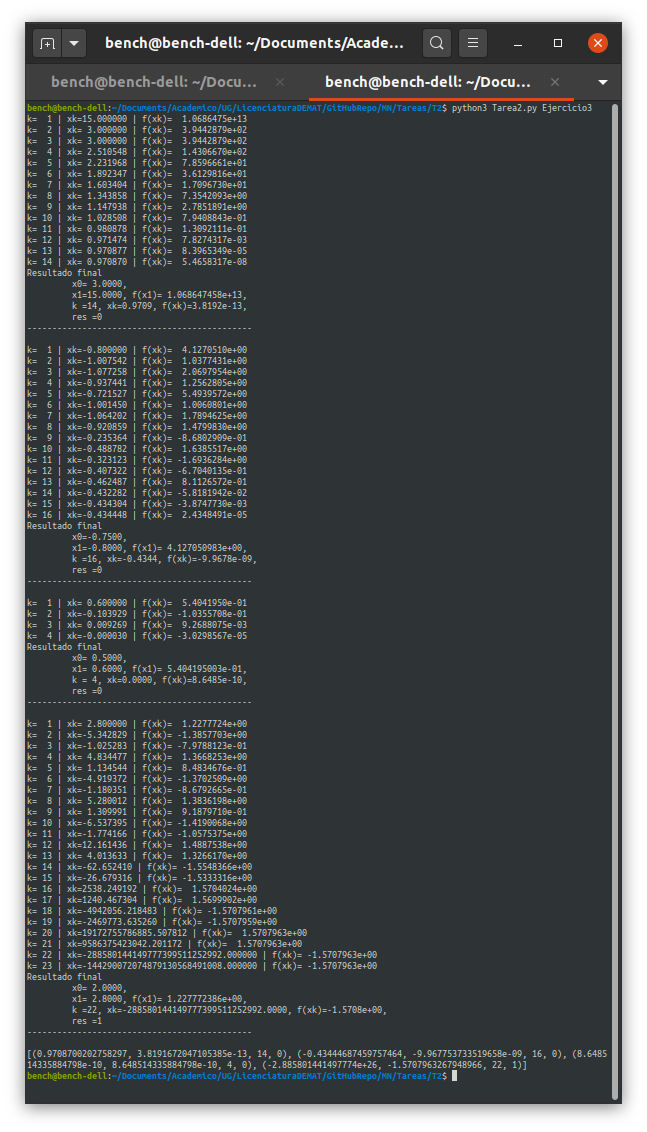
\includegraphics{assets/E3-1.png}
		\caption{Evidencia Ejecucion}
	\end{figure}
















\newpage
    \hypertarget{ejercicio-4}{%
\subsection{Ejercicio 4}\label{ejercicio-4}}

		\textbf{Respuesta} Es posible que este metodo encuentre puntos que no
	corresponden a las raices, pero estos son facilmente identificables en
	la grafica. Este error se da porque no se filtra el resultado res del
	metodo de la secante.

		\begin{tcolorbox}[breakable, size=fbox, boxrule=1pt, pad at break*=1mm,colback=cellbackground, colframe=cellborder]
	\prompt{In}{incolor}{73}{\boxspacing}
	\begin{Verbatim}[commandchars=\\\{\}]
	\PY{k}{def} \PY{n+nf}{f\PYZus{}polinomio}\PY{p}{(}\PY{n}{coef}\PY{p}{)}\PY{p}{:}
		\PY{l+s+sd}{\PYZdq{}\PYZdq{}\PYZdq{} Funcion que genera una funcion polinomial de una variable dados sus coeficientes \PYZdq{}\PYZdq{}\PYZdq{}}
		\PY{k}{return} \PY{n}{f}
	\PY{k}{def} \PY{n+nf}{eta\PYZus{}Teorema1}\PY{p}{(}\PY{n}{coef}\PY{p}{)}\PY{p}{:}
		\PY{l+s+sd}{\PYZdq{}\PYZdq{}\PYZdq{} Funcion que calcula la variable eta del T1 \PYZdq{}\PYZdq{}\PYZdq{}}
		\PY{k}{return} \PY{n+nb}{max}\PY{p}{(}\PY{p}{[}\PY{n+nb}{abs}\PY{p}{(}\PY{n}{ak}\PY{o}{/}\PY{n}{coef}\PY{p}{[}\PY{l+m+mi}{0}\PY{p}{]}\PY{p}{)} \PY{k}{for} \PY{n}{ak} \PY{o+ow}{in} \PY{n}{coef}\PY{p}{[}\PY{l+m+mi}{1}\PY{p}{:}\PY{p}{]}\PY{p}{]}\PY{p}{)}
	\PY{k}{def} \PY{n+nf}{Teorema1}\PY{p}{(}\PY{n}{f}\PY{p}{,} \PY{n}{eta}\PY{p}{,}\PY{o}{/}\PY{p}{,} \PY{n}{metodo}\PY{o}{=}\PY{n}{metodo\PYZus{}secante}\PY{p}{)}\PY{p}{:}
		\PY{l+s+sd}{\PYZdq{}\PYZdq{}\PYZdq{} Impementacion de los conceptos del T1 \PYZdq{}\PYZdq{}\PYZdq{}}
		\PY{n}{t} \PY{o}{=} \PY{l+m+mf}{2.2e\PYZhy{}16}\PY{o}{*}\PY{o}{*}\PY{p}{(}\PY{l+m+mi}{1}\PY{o}{/}\PY{l+m+mi}{2}\PY{p}{)} \PY{c+c1}{\PYZsh{} Tolerancia}
		\PY{n}{p} \PY{o}{=} \PY{l+m+mf}{1.0e\PYZhy{}2} \PY{c+c1}{\PYZsh{} Paso entre pruebas; definido arbitrariamente en funcio de la visualizacion de la grafica}
		\PY{n}{N} \PY{o}{=} \PY{l+m+mi}{40}     \PY{c+c1}{\PYZsh{} Por iluminacion divina}
		
		\PY{n}{I} \PY{o}{=} \PY{p}{[}\PY{o}{\PYZhy{}}\PY{n+nb}{int}\PY{p}{(}\PY{n}{eta}\PY{o}{+}\PY{l+m+mi}{1}\PY{p}{)}\PY{p}{,} \PY{n+nb}{int}\PY{p}{(}\PY{n}{eta}\PY{o}{+}\PY{l+m+mi}{1}\PY{p}{)}\PY{p}{]} \PY{c+c1}{\PYZsh{} Limite del Teorema 1}
		\PY{n}{r\PYZus{}min} \PY{o}{=} \PY{n}{metodo}\PY{p}{(}\PY{n}{f}\PY{p}{,} \PY{n}{I}\PY{p}{[}\PY{l+m+mi}{0}\PY{p}{]}\PY{p}{,} \PY{n}{I}\PY{p}{[}\PY{l+m+mi}{0}\PY{p}{]}\PY{o}{+}\PY{l+m+mi}{2}\PY{p}{,} \PY{n}{t}\PY{p}{,} \PY{n}{N}\PY{p}{,} \PY{k+kc}{False}\PY{p}{)}\PY{p}{[}\PY{l+m+mi}{0}\PY{p}{]}
		\PY{n}{r\PYZus{}max} \PY{o}{=} \PY{n}{metodo}\PY{p}{(}\PY{n}{f}\PY{p}{,} \PY{n}{I}\PY{p}{[}\PY{l+m+mi}{1}\PY{p}{]}\PY{o}{\PYZhy{}}\PY{l+m+mi}{2}\PY{p}{,} \PY{n}{I}\PY{p}{[}\PY{l+m+mi}{1}\PY{p}{]}\PY{p}{,} \PY{n}{t}\PY{p}{,} \PY{n}{N}\PY{p}{,} \PY{k+kc}{False}\PY{p}{)}\PY{p}{[}\PY{l+m+mi}{0}\PY{p}{]}
		\PY{n}{ret} \PY{o}{=} \PY{p}{[}\PY{n}{r\PYZus{}min}\PY{p}{]}
		
		\PY{k}{if} \PY{o+ow}{not} \PY{p}{(}\PY{n}{r\PYZus{}max} \PY{o}{\PYZlt{}}\PY{o}{=} \PY{n}{r\PYZus{}min}\PY{p}{)}\PY{p}{:} \PY{c+c1}{\PYZsh{} Buscamos mas}
		    \PY{n}{xk} \PY{o}{=} \PY{n}{r\PYZus{}min}\PY{o}{+}\PY{n}{p}
		    \PY{n}{fa} \PY{o}{=} \PY{n}{f}\PY{p}{(}\PY{n}{r\PYZus{}min}\PY{o}{+}\PY{n}{p}\PY{p}{)} \PY{c+c1}{\PYZsh{} Evaluacion de raiz anterior}
		    
		    \PY{k}{while} \PY{n}{xk} \PY{o}{\PYZlt{}} \PY{n}{r\PYZus{}max}\PY{p}{:} \PY{c+c1}{\PYZsh{} Iteracion principal}
		        \PY{n}{xk} \PY{o}{+}\PY{o}{=} \PY{n}{p} \PY{c+c1}{\PYZsh{} Avanzamos un paso entre rmin y rmax}
		        \PY{k}{if} \PY{n}{f}\PY{p}{(}\PY{n}{xk}\PY{p}{)}\PY{o}{*}\PY{n}{fa} \PY{o}{\PYZlt{}} \PY{l+m+mi}{0}\PY{p}{:}  \PY{c+c1}{\PYZsh{} Buscamos cambio de signo}
		            \PY{n}{ret}\PY{o}{.}\PY{n}{append}\PY{p}{(}\PY{n}{metodo}\PY{p}{(}\PY{n}{f}\PY{p}{,}\PY{n}{xk}\PY{o}{\PYZhy{}}\PY{n}{p}\PY{p}{,}\PY{n}{xk}\PY{p}{,}\PY{n}{t}\PY{p}{,} \PY{n}{N}\PY{p}{,} \PY{k+kc}{False}\PY{p}{)}\PY{p}{[}\PY{l+m+mi}{0}\PY{p}{]}\PY{p}{)}
		            \PY{n}{fa} \PY{o}{=} \PY{n}{f}\PY{p}{(}\PY{n}{xk}\PY{p}{)}
		    \PY{n}{ret}\PY{o}{.}\PY{n}{append}\PY{p}{(}\PY{n}{r\PYZus{}max}\PY{p}{)}
		
		\PY{k}{return} \PY{n}{ret}
	\end{Verbatim}
	\end{tcolorbox}

		\begin{tcolorbox}[breakable, size=fbox, boxrule=1pt, pad at break*=1mm,colback=cellbackground, colframe=cellborder]
	\prompt{In}{incolor}{74}{\boxspacing}
		\begin{Verbatim}[commandchars=\\\{\}]
			\PY{k}{def} \PY{n+nf}{Ejercicio4}\PY{p}{(}\PY{p}{)}\PY{p}{:}
				\PY{n}{coef} \PY{o}{=} \PY{p}{[}\PY{l+m+mi}{6}\PY{p}{,} \PY{o}{\PYZhy{}}\PY{l+m+mi}{25}\PY{p}{,} \PY{o}{\PYZhy{}}\PY{l+m+mi}{24}\PY{p}{,} \PY{l+m+mi}{110}\PY{p}{,} \PY{o}{\PYZhy{}}\PY{l+m+mi}{72}\PY{p}{,} \PY{l+m+mi}{320}\PY{p}{]}
				\PY{n}{eta} \PY{o}{=} \PY{n}{eta\PYZus{}Teorema1}\PY{p}{(}\PY{n}{coef}\PY{p}{)}
				\PY{n}{f} \PY{o}{=} \PY{n}{f\PYZus{}polinomio}\PY{p}{(}\PY{n}{coef}\PY{p}{)}
				\PY{n}{raices} \PY{o}{=} \PY{n}{Teorema1}\PY{p}{(}\PY{n}{f}\PY{p}{,} \PY{n}{eta}\PY{p}{)}

				\PY{l+s+sd}{\PYZdq{}\PYZdq{}\PYZdq{} Grafica del resultado\PYZdq{}\PYZdq{}\PYZdq{}}
				
				\PY{k}{return} \PY{n}{raices}
				
			\PY{n}{Ejercicio4}\PY{p}{(}\PY{p}{)}
		\end{Verbatim}
	\end{tcolorbox}

		\begin{center}
			\adjustimage{max size={0.7\linewidth}{0.7\paperheight}}{assets/output_23_0.png}
		\end{center}
		{ \hspace*{\fill} \\}		
		\hypertarget{como-ejecutar}{%
	\subsubsection{Como ejecutar}\label{como-ejecutar}}

		\href{https://colab.research.google.com/gist/BenchHPZ/.../---.ipynb}{GoogleColab}

	Para ejecutar este ejercicio en \textbf{consola} es importante ubicarse
	en la misma carpeta del
	\href{https://github.com/BenchHPZ/UG-Compu/blob/master/MN/Tareas/T2/Tarea2.py}{archivo
	\texttt{Tarea2.py}} y ejecutar el siguiente comando en consola

	\begin{verbatim}
	python3 Tarea2.py Ejercicio4
	\end{verbatim}

	Este programa no espera recibir argumento alguno. La salida debe ser
	similar a la siguiente imagen

	\begin{figure}
	\centering
	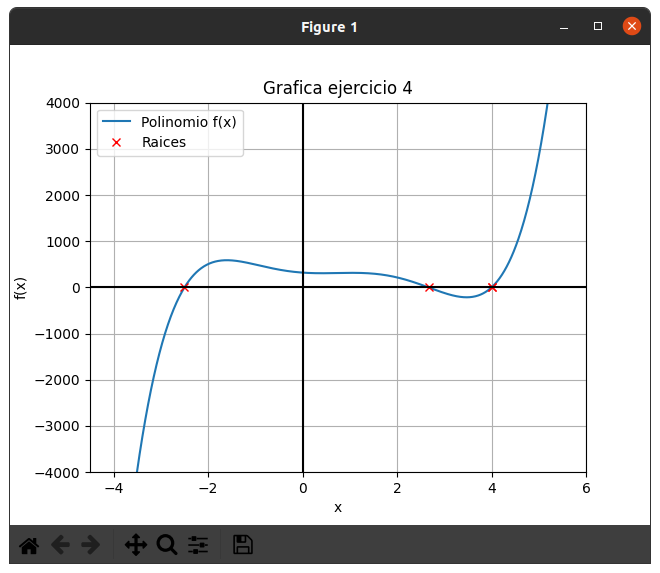
\includegraphics{assets/E4-1.png}
	\caption{Evidencia Ejecucion}
	\end{figure}












\newpage
    \hypertarget{ejercicio-5}{%
\subsection{Ejercicio 5}\label{ejercicio-5}}

    \textbf{Respuesta}

    \begin{tcolorbox}[breakable, size=fbox, boxrule=1pt, pad at break*=1mm,colback=cellbackground, colframe=cellborder]
\prompt{In}{incolor}{75}{\boxspacing}
\begin{Verbatim}[commandchars=\\\{\}]
\PY{k}{def} \PY{n+nf}{metodo\PYZus{}horner}\PY{p}{(}\PY{n}{n}\PY{p}{,} \PY{n}{a}\PY{p}{,} \PY{n}{x0}\PY{p}{,}\PY{o}{/}\PY{p}{,}\PY{n}{v}\PY{o}{=}\PY{k+kc}{True}\PY{p}{,} \PY{n}{td}\PY{o}{=}\PY{n}{np}\PY{o}{.}\PY{n}{float64}\PY{p}{)}\PY{p}{:}
    \PY{l+s+sd}{\PYZdq{}\PYZdq{}\PYZdq{} Implementacion del metodo de horner, basado}
\PY{l+s+sd}{    en el pseudocodigo del documento de la tarea.}
\PY{l+s+sd}{        Input}
\PY{l+s+sd}{            n := Grado del polinomio}
\PY{l+s+sd}{            a := Arreglo de coeficientes}
\PY{l+s+sd}{            x0 := Punto inicial del metodo}
\PY{l+s+sd}{        Output}
\PY{l+s+sd}{            (y, b)}
\PY{l+s+sd}{            y := evaluacion final}
\PY{l+s+sd}{            b := coeficientes de polinomio asociado}
\PY{l+s+sd}{    \PYZdq{}\PYZdq{}\PYZdq{}}
    \PY{n}{x0} \PY{o}{=} \PY{n}{td}\PY{p}{(}\PY{n}{x0}\PY{p}{)}
    \PY{n}{a} \PY{o}{=} \PY{p}{[}\PY{n}{td}\PY{p}{(}\PY{n}{c}\PY{p}{)} \PY{k}{for} \PY{n}{c} \PY{o+ow}{in} \PY{n}{a}\PY{p}{]} \PY{c+c1}{\PYZsh{} Normalizar el tipo de dato}
    \PY{n}{b} \PY{o}{=} \PY{n}{a}\PY{p}{[}\PY{p}{:}\PY{p}{]}               \PY{c+c1}{\PYZsh{} Reservar memoria xP}
    \PY{k}{for} \PY{n}{k} \PY{o+ow}{in} \PY{n+nb}{range}\PY{p}{(}\PY{l+m+mi}{1}\PY{p}{,}\PY{n}{n}\PY{p}{)}\PY{p}{:}
        \PY{n}{b}\PY{p}{[}\PY{n}{k}\PY{p}{]} \PY{o}{=} \PY{n}{a}\PY{p}{[}\PY{n}{k}\PY{p}{]} \PY{o}{\PYZhy{}} \PY{n}{b}\PY{p}{[}\PY{n}{k}\PY{o}{\PYZhy{}}\PY{l+m+mi}{1}\PY{p}{]}\PY{o}{*}\PY{n}{x0}
    \PY{k}{return} \PY{n}{a}\PY{p}{[}\PY{o}{\PYZhy{}}\PY{l+m+mi}{1}\PY{p}{]}\PY{o}{\PYZhy{}}\PY{n}{b}\PY{p}{[}\PY{o}{\PYZhy{}}\PY{l+m+mi}{2}\PY{p}{]}\PY{o}{*}\PY{n}{x0}
\end{Verbatim}
\end{tcolorbox}

    \begin{tcolorbox}[breakable, size=fbox, boxrule=1pt, pad at break*=1mm,colback=cellbackground, colframe=cellborder]
\prompt{In}{incolor}{76}{\boxspacing}
\begin{Verbatim}[commandchars=\\\{\}]
	\PY{k}{def} \PY{n+nf}{Ejercicio5}\PY{p}{(}\PY{n}{v}\PY{o}{=}\PY{k+kc}{True}\PY{p}{)}\PY{p}{:}
		\PY{l+s+sd}{\PYZdq{}\PYZdq{}\PYZdq{} Ejercicio 6 de Tarea 2\PYZdq{}\PYZdq{}\PYZdq{}}
		\PY{n}{dt} \PY{o}{=} \PY{n}{np}\PY{o}{.}\PY{n}{float64}
		\PY{n}{coef} \PY{o}{=} \PY{p}{[}\PY{l+m+mi}{6}\PY{p}{,} \PY{o}{\PYZhy{}}\PY{l+m+mi}{25}\PY{p}{,} \PY{o}{\PYZhy{}}\PY{l+m+mi}{24}\PY{p}{,} \PY{l+m+mi}{110}\PY{p}{,} \PY{o}{\PYZhy{}}\PY{l+m+mi}{72}\PY{p}{,} \PY{l+m+mi}{320}\PY{p}{]}
		\PY{n}{coef\PYZus{}dx} \PY{o}{=} \PY{p}{[}\PY{l+m+mi}{30}\PY{p}{,} \PY{o}{\PYZhy{}}\PY{l+m+mi}{100}\PY{p}{,} \PY{o}{\PYZhy{}}\PY{l+m+mi}{72}\PY{p}{,} \PY{l+m+mi}{220}\PY{p}{,} \PY{o}{\PYZhy{}}\PY{l+m+mi}{72}\PY{p}{]}
		\PY{n}{muestras} \PY{o}{=} \PY{l+m+mi}{20}
		
		\PY{n}{Ep} \PY{o}{=} \PY{l+m+mi}{0}\PY{p}{;} \PY{n}{Ed} \PY{o}{=} \PY{l+m+mi}{0}
		\PY{n}{xs} \PY{o}{=} \PY{n}{np}\PY{o}{.}\PY{n}{linspace}\PY{p}{(}\PY{o}{\PYZhy{}}\PY{l+m+mi}{5}\PY{p}{,} \PY{l+m+mi}{5}\PY{p}{,} \PY{n}{num}\PY{o}{=}\PY{n}{muestras}\PY{p}{,} \PY{n}{dtype}\PY{o}{=}\PY{n}{dt}\PY{p}{)}
		\PY{n}{f} \PY{o}{=} \PY{n}{f\PYZus{}polinomio}\PY{p}{(}\PY{n}{coef}\PY{p}{)}
		\PY{n}{df} \PY{o}{=} \PY{n}{f\PYZus{}polinomio}\PY{p}{(}\PY{n}{coef\PYZus{}dx}\PY{p}{)}
		
		\PY{k}{for} \PY{n}{k} \PY{o+ow}{in} \PY{n+nb}{range}\PY{p}{(}\PY{l+m+mi}{20}\PY{p}{)}\PY{p}{:}
		    \PY{n}{px}  \PY{o}{=} \PY{n}{metodo\PYZus{}horner}\PY{p}{(}\PY{n+nb}{len}\PY{p}{(}\PY{n}{coef}\PY{p}{)}\PY{p}{,} \PY{n}{coef}\PY{p}{,} \PY{n}{xs}\PY{p}{[}\PY{n}{k}\PY{p}{]}\PY{p}{)}
		    \PY{n}{dpx} \PY{o}{=} \PY{n}{metodo\PYZus{}horner}\PY{p}{(}\PY{n+nb}{len}\PY{p}{(}\PY{n}{coef}\PY{p}{)}\PY{o}{\PYZhy{}}\PY{l+m+mi}{1}\PY{p}{,} \PY{n}{coef}\PY{p}{,} \PY{n}{xs}\PY{p}{[}\PY{n}{k}\PY{p}{]}\PY{p}{)}    
		    \PY{n}{dif\PYZus{}p} \PY{o}{=} \PY{p}{(}\PY{n}{f}\PY{p}{(}\PY{n}{xs}\PY{p}{[}\PY{n}{k}\PY{p}{]}\PY{p}{)} \PY{o}{\PYZhy{}} \PY{n}{px}\PY{p}{)}
		    \PY{n}{dif\PYZus{}d} \PY{o}{=} \PY{p}{(}\PY{n}{df}\PY{p}{(}\PY{n}{xs}\PY{p}{[}\PY{n}{k}\PY{p}{]}\PY{p}{)} \PY{o}{\PYZhy{}} \PY{n}{dpx}\PY{p}{)}
		    
		    \PY{n}{Ep} \PY{o}{+}\PY{o}{=} \PY{n+nb}{abs}\PY{p}{(}\PY{n}{dif\PYZus{}p}\PY{p}{)}
		    \PY{n}{Ed} \PY{o}{+}\PY{o}{=} \PY{n+nb}{abs}\PY{p}{(}\PY{n}{dif\PYZus{}d}\PY{p}{)}
		    \PY{k}{if} \PY{n}{v}\PY{p}{:} \PY{n+nb}{print}\PY{p}{(}\PY{l+s+sa}{...}\PY{p}{)}
		\PY{k}{if} \PY{n}{v}\PY{p}{:} \PY{n+nb}{print}\PY{p}{(}\PY{l+s+sa}{f}\PY{l+s+s1}{\PYZsq{}}\PY{l+s+se}{\PYZbs{}n}\PY{l+s+s1}{\PYZhy{}\PYZhy{}\PYZhy{}FIN\PYZhy{}\PYZhy{}\PYZhy{}}\PY{l+s+se}{\PYZbs{}n}\PY{l+s+s1}{\PYZsq{}}
		            \PY{l+s+sa}{f}\PY{l+s+s1}{\PYZsq{}}\PY{l+s+s1}{Ep=}\PY{l+s+si}{\PYZob{}}\PY{n}{Ep}\PY{o}{/}\PY{l+m+mi}{20}\PY{l+s+si}{\PYZcb{}}\PY{l+s+s1}{ | Ed=}\PY{l+s+si}{\PYZob{}}\PY{n}{Ed}\PY{o}{/}\PY{l+m+mi}{20}\PY{l+s+si}{\PYZcb{}}\PY{l+s+s1}{\PYZsq{}}\PY{p}{)}
		\PY{k}{return} \PY{p}{(}\PY{n}{Ep}\PY{o}{/}\PY{l+m+mi}{20}\PY{p}{,} \PY{n}{Ed}\PY{o}{/}\PY{l+m+mi}{20}\PY{p}{)}


	\PY{n+nb}{print}\PY{p}{(}\PY{n}{Ejercicio5}\PY{p}{(}\PY{p}{)}\PY{p}{)}
\end{Verbatim}
\end{tcolorbox}

\begin{multicols}{2}\scriptsize
    \begin{Verbatim}[commandchars=\\\{\}]
k=  0
  px= 2835.000000 | dif\_p=-30780.000000
 dpx= 2835.000000 | dif\_d=25443.000000
k=  1
  px=  788.425780 | dif\_p=-16561.514891
 dpx=  788.425780 | dif\_d=17684.557377
k=  2
  px=  -45.844732 | dif\_p=-7979.828634
 dpx=  -45.844732 | dif\_d=11417.915526
k=  3
  px= -212.626585 | dif\_p=-3208.668531
 dpx= -212.626585 | dif\_d= 6658.427630
k=  4
  px=  -84.690012 | dif\_p= -857.931844
 dpx=  -84.690012 | dif\_d= 3304.650249
k=  5
  px=  108.161574 | dif\_p=   84.470201
 dpx=  108.161574 | dif\_d= 1167.421318
k=  6
  px=  250.013584 | dif\_p=  310.768406
 dpx=  250.013584 | dif\_d=   -1.061857
k=  7
  px=  309.762253 | dif\_p=  251.491600
 dpx=  309.762253 | dif\_d= -478.164598
k=  8
  px=  312.036645 | dif\_p=  133.622630
 dpx=  312.036645 | dif\_d= -541.736862
k=  9
  px=  308.120655 | dif\_p=   38.754355
 dpx=  308.120655 | dif\_d= -441.035243
k= 10
  px=  346.875010 | dif\_p=  -38.754355
 dpx=  346.875010 | dif\_d= -367.644970
k= 11
  px=  445.659275 | dif\_p= -133.622630
 dpx=  445.659275 | dif\_d= -426.401918
k= 12
  px=  561.253853 | dif\_p= -251.491600
 dpx=  561.253853 | dif\_d= -606.314603
k= 13
  px=  560.781990 | dif\_p= -310.768406
 dpx=  560.781990 | dif\_d= -751.486190
k= 14
  px=  192.631775 | dif\_p=  -84.470201
 dpx=  192.631775 | dif\_d= -532.036491
k= 15
  px= -942.621856 | dif\_p=  857.931844
 dpx= -942.621856 | dif\_d=  584.976028
k= 16
  px=-3421.295116 | dif\_p= 3208.668531
 dpx=-3421.295116 | dif\_d= 3364.632245
k= 17
  px=-8025.673366 | dif\_p= 7979.828634
 dpx=-8025.673366 | dif\_d= 8833.230383
k= 18
  px=-15773.089111 | dif\_p=16561.514891
 dpx=-15773.089111 | dif\_d=18307.364002
k= 19
  px=-27945.000000 | dif\_p=30780.000000
 dpx=-27945.000000 | dif\_d=33423.000000

---FIN---
Ep=6020.705109125281 | Ed=6716.752874460997
(6020.705109125281, 6716.752874460997)
    \end{Verbatim}
\end{multicols}

    \begin{tcolorbox}[breakable, size=fbox, boxrule=1pt, pad at break*=1mm,colback=cellbackground, colframe=cellborder]
\prompt{In}{incolor}{77}{\boxspacing}
\begin{Verbatim}[commandchars=\\\{\}]
\PY{c+c1}{\PYZsh{} alternativas}
\PY{l+s+sd}{\PYZdq{}\PYZdq{}\PYZdq{} Alternativa a np.linspace\PYZdq{}\PYZdq{}\PYZdq{}}
\PY{k}{def} \PY{n+nf}{linspace}\PY{p}{(}\PY{n}{start}\PY{p}{,} \PY{n}{stop}\PY{p}{,} \PY{n}{n}\PY{p}{)}\PY{p}{:}
    \PY{l+s+sd}{\PYZdq{}\PYZdq{}\PYZdq{} Programa que entrega un arreglo de numeros}
\PY{l+s+sd}{    equitativamnte espaciado de n elementos empe\PYZus{}}
\PY{l+s+sd}{    zando en start y hasta stop.}
\PY{l+s+sd}{    }
\PY{l+s+sd}{    \PYZus{}Doctest}
\PY{l+s+sd}{        \PYZgt{}\PYZgt{}\PYZgt{} linspace(\PYZhy{}5,5,3)}
\PY{l+s+sd}{        [\PYZhy{}5.0, 0.0, 5.0]}
\PY{l+s+sd}{    \PYZdq{}\PYZdq{}\PYZdq{}}
    \PY{n}{step} \PY{o}{=} \PY{p}{(}\PY{n}{stop}\PY{o}{\PYZhy{}}\PY{n}{start}\PY{p}{)}\PY{o}{/}\PY{p}{(}\PY{n}{n}\PY{o}{\PYZhy{}}\PY{l+m+mi}{1}\PY{p}{)}
    \PY{k}{return} \PY{p}{[}\PY{n}{start}\PY{o}{+}\PY{n}{step}\PY{o}{*}\PY{p}{(}\PY{n}{i}\PY{p}{)} \PY{k}{for} \PY{n}{i} \PY{o+ow}{in} \PY{n+nb}{range}\PY{p}{(}\PY{n}{n}\PY{p}{)}\PY{p}{]}
\end{Verbatim}
\end{tcolorbox}

    \hypertarget{ejercicio-5}{%
\subsubsection{Ejercicio 5}\label{ejercicio-5}}

    \href{https://colab.research.google.com/gist/BenchHPZ/.../---.ipynb}{GoogleColab}

Para ejecutar este ejercicio en \textbf{consola} es importante ubicarse
en la misma carpeta del
\href{https://github.com/BenchHPZ/UG-Compu/blob/master/MN/Tareas/T2/Tarea2.py}{archivo
\texttt{Tarea2.py}} y ejecutar el siguiente comando en consola

\begin{verbatim}
python3 Tarea2.py Ejercicio5
\end{verbatim}

Este programa no espera recibir argumento alguno. La salida debe ser
similar a la siguiente imagen

\begin{figure}
\centering
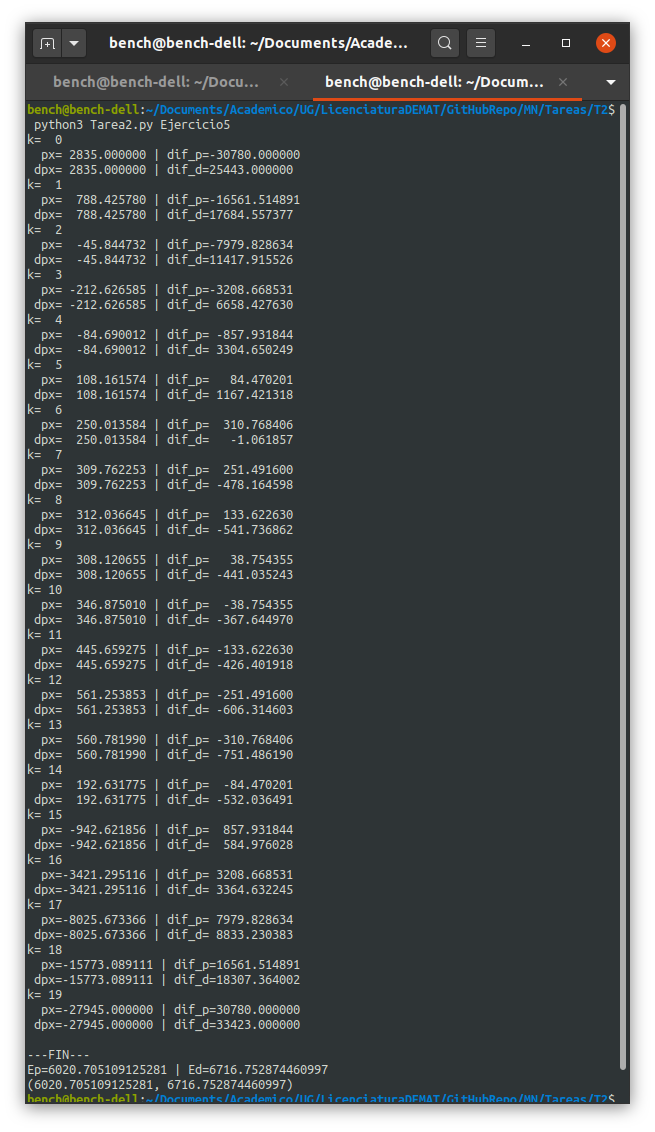
\includegraphics{assets/E5-1.png}
\caption{Evidencia Ejecucion}
\end{figure}


    % Add a bibliography block to the postdoc
    
    
    
\end{document}
